%%%%%%%%%%%%%%%%%%%%%%%%%%%%%%%%%%%%%%%%%%%%%%%%%%%%%%%%%%%%%%%%%%%%%%%%%%%%%%%
%                       CARREGA DE LA CLASSE DE DOCUMENT                      %
%                                                                             %
% Les opcions admissibles son:                                                %
%      12pt / 11pt            (cos dels tipus de lletra; no feu servir 10pt)  %
%                                                                             %
% catalan/spanish/english     (llengua principal del treball)                 %
%                                                                             % 
% french/italian/german...    (si necessiteu fer servir alguna altra llengua) %
%                                                                             %
% listoffigures               (El document inclou un Index de figures)        %
% listoftables                (El document inclou un Index de taules)         %
% listofquadres               (El document inclou un Index de quadres)        %
% listofalgorithms            (El document inclou un Index d'algorismes)      %
%                                                                             %
%%%%%%%%%%%%%%%%%%%%%%%%%%%%%%%%%%%%%%%%%%%%%%%%%%%%%%%%%%%%%%%%%%%%%%%%%%%%%%%

\documentclass[11pt,spanish,listoffigures,listoftables]{tfgetsinf}

%%%%%%%%%%%%%%%%%%%%%%%%%%%%%%%%%%%%%%%%%%%%%%%%%%%%%%%%%%%%%%%%%%%%%%%%%%%%%%%
%                     CODIFICACIO DEL FITXER FONT                             %
%                                                                             %
%    windows fa servir normalment 'ansinew'                                   %
%    amb linux es possible que siga 'latin1' o 'latin9'                       %
%    Pero el mes recomanable es fer servir utf8 (unicode 8)                   %
%                                          (si el vostre editor ho permet)    % 
%%%%%%%%%%%%%%%%%%%%%%%%%%%%%%%%%%%%%%%%%%%%%%%%%%%%%%%%%%%%%%%%%%%%%%%%%%%%%%%

\usepackage[utf8]{inputenc} 

%%%%%%%%%%%%%%%%%%%%%%%%%%%%%%%%%%%%%%%%%%%%%%%%%%%%%%%%%%%%%%%%%%%%%%%%%%%%%%%
%                        ALTRES PAQUETS I DEFINICIONS                         %
%                                                                             %
% Carregueu aci els paquets que necessiteu i declareu les comandes i entorns  %
%                                          (aquesta seccio pot ser buida)     %
%%%%%%%%%%%%%%%%%%%%%%%%%%%%%%%%%%%%%%%%%%%%%%%%%%%%%%%%%%%%%%%%%%%%%%%%%%%%%%%



%%%%%%%%%%%%%%%%%%%%%%%%%%%%%%%%%%%%%%%%%%%%%%%%%%%%%%%%%%%%%%%%%%%%%%%%%%%%%%%
%                        DADES DEL TREBALL                                    %
%                                                                             %
% titol, alumne, tutor i curs academic                                        %
%%%%%%%%%%%%%%%%%%%%%%%%%%%%%%%%%%%%%%%%%%%%%%%%%%%%%%%%%%%%%%%%%%%%%%%%%%%%%%%

\title{Gestor de turnos  \\
         de teletrabajo}
\author{Julián Rincón Morales}
\tutor{Pau Miñana Climent}
\curs{2020-2021}

%%%%%%%%%%%%%%%%%%%%%%%%%%%%%%%%%%%%%%%%%%%%%%%%%%%%%%%%%%%%%%%%%%%%%%%%%%%%%%%
%                     PARAULES CLAU/PALABRAS CLAVE/KEY WORDS                  %
%                                                                             %
% Independentment de la llengua del treball, s'hi han d'incloure              %
% les paraules clau i el resum en els tres idiomes                            %
%%%%%%%%%%%%%%%%%%%%%%%%%%%%%%%%%%%%%%%%%%%%%%%%%%%%%%%%%%%%%%%%%%%%%%%%%%%%%%%

\keywords{teletreball, organització, torn, node, quasar, sequelize, mariadb, docker, express, rest api} % Paraules clau 
         {teletrabajo, organizacion, turno, node, quasar, sequelize, mariadb, docker, express, rest api}              % Palabras clave
         {telework,  setup, turn, shift, node, quasar, sequelize, mariadb, docker, express, rest api}        % Key words

%%%%%%%%%%%%%%%%%%%%%%%%%%%%%%%%%%%%%%%%%%%%%%%%%%%%%%%%%%%%%%%%%%%%%%%%%%%%%%%
%                              INICI DEL DOCUMENT                             %
%%%%%%%%%%%%%%%%%%%%%%%%%%%%%%%%%%%%%%%%%%%%%%%%%%%%%%%%%%%%%%%%%%%%%%%%%%%%%%%

\begin{document}

%%%%%%%%%%%%%%%%%%%%%%%%%%%%%%%%%%%%%%%%%%%%%%%%%%%%%%%%%%%%%%%%%%%%%%%%%%%%%%%
%              RESUMS DEL TFG EN VALENCIA, CASTELLA I ANGLES                  %
%%%%%%%%%%%%%%%%%%%%%%%%%%%%%%%%%%%%%%%%%%%%%%%%%%%%%%%%%%%%%%%%%%%%%%%%%%%%%%%

\begin{abstract}
Gestor de torns de teletreball és una eina per a organitzar els torns en els quals el personal dels diferents departaments d'una empresa s'alternen per a teletreballar.
Per al client bàsic, s'ofereix un calendari on pot confirmar els torns que li són assignats o sol·licitar canvi a un altre company.
També té visibilitat sobre els torns de la seua pròpia àrea per a poder sol·licitar el canvi.
A mes pot obtindre una còpia del calendari en pdf per a imprimir-la posteriorment o emmagatzemar-la.
El gestor del departament pot obtindre un informe amb gràfics del personal que està al seu càrrec.
L'administrador de l'aplicació té una interfície per a poder modificar els valors de l'aplicació.
\end{abstract}
\begin{abstract}[spanish]
Gestor de turnos de teletrabajo es una herramienta para organizar los turnos en los que el personal de los distintos departamentos de una empresa se turnan para teletrabajar.
Para el cliente básico, se ofrece un calendario donde puede confirmar los turnos que le son asignados o solicitar cambio a otro compañero.
También tiene visibilidad sobre los turnos de su propia area para poder solicitar el cambio.
Ademas puede obtener una copia del calendario en pdf para imprimirla posteriormente o almacenarla.
El gestor del departamento puede obtener un informe con graficos del personal que está a su cargo.
El administrador de la aplicación tiene un interfaz para poder modificar los valores de la aplicación.
\end{abstract}
\begin{abstract}[english]
Telework Shift Manager is a tool to organize shifts in which the personnel of the different departments of a company takes turns to telework.
For the basic client, a calendar is offered where you can confirm the shifts that are assigned to you or request a change from another colleague.
You also have visibility on the shifts in your area to be able to request the change.
You can also get a copy of the calendar in pdf to print it later or store it.
The department manager can obtain a report with graphs of the personnel who are in charge.
The application manager has an interface to be able to modify the application settings.
\end{abstract}

%%%%%%%%%%%%%%%%%%%%%%%%%%%%%%%%%%%%%%%%%%%%%%%%%%%%%%%%%%%%%%%%%%%%%%%%%%%%%%%
%                              CONTINGUT DEL TREBALL                          %
%%%%%%%%%%%%%%%%%%%%%%%%%%%%%%%%%%%%%%%%%%%%%%%%%%%%%%%%%%%%%%%%%%%%%%%%%%%%%%%

\mainmatter

%%%%%%%%%%%%%%%%%%%%%%%%%%%%%%%%%%%%%%%%%%%%%%%%%%%%%%%%%%%%%%%%%%%%%%%%%%%%%%%
%                                  INTRODUCCIO                                %
%%%%%%%%%%%%%%%%%%%%%%%%%%%%%%%%%%%%%%%%%%%%%%%%%%%%%%%%%%%%%%%%%%%%%%%%%%%%%%%

\chapter{Introducci\'o}

Al incorporar el teletrabajo en nuestra forma de vida, muchas empresas que no tenían ningún sistema de turnos porque no les hacía falta, han visto que no disponen de herramientas para coordinar los diversos grupos de trabajo.

Muchas de estas empresas optan por usar el calendario del correo o  una hoja excel, en ocasiones generando descoordinación al no tener un sistema fácil donde poder marcar y modificar los días en los que el personal debe acudir de forma presencial.

También es posible que no se distribuyan de forma equitativa los turnos, pudiendo generar malestar entre los compañeros.

% \section{Motivaci\'o}
%
%Lograr una aplicación que muestre  
%
\section{Objectius}

El objetivo de este proyecto es crear una aplicación que de forma rápida permita configurar las jornadas de teletrabajo, y dotar a los responsables de los mismos estadísticas del personal a su cargo.

Que puedan consultar de forma rápida si al día siguiente es turno presencial o no, y guardarse una copia de los turnos del mes para poder consultarlo posteriormente. 


%\section{Notes bibliografiques} %%%%% Opcional

%????? ????????????? ????????????? ????????????? ????????????? ?????????????

%%%%%%%%%%%%%%%%%%%%%%%%%%%%%%%%%%%%%%%%%%%%%%%%%%%%%%%%%%%%%%%%%%%%%%%%%%%%%%%
%                         CAPITOLS (tants com calga)                          %
%%%%%%%%%%%%%%%%%%%%%%%%%%%%%%%%%%%%%%%%%%%%%%%%%%%%%%%%%%%%%%%%%%%%%%%%%%%%%%%

\chapter{Estado del arte}

El ORM (object-relational mapping) Sequelize, desde su versión 4, permite el uso de clases ES6, por lo que se ha usado una clase básica con los parametros comunes, eliminando codigo duplicado.

Se ha integrado CI/CD en la creación de esta documentación, a través de github actions, compilando el documento al realizar un push en el respositorio.

El uso de Sonarqube ha limitado el código duplicado, llegando a ser inexistente en la parte del frontend.

Quasar es una herramienta basada en vue que permite crear itnerfaces gráficos de forma sencilla.

Docker es una virtualización muy ligera que combinada con docker-compose permite crear el despliegue de la aplicación en multiples sistemas de forma muy sencilla.

Google cloud es uno de los servidores donde podemos desplegarlo, viendo las posibilidades con aplicación móvil y sin ella.

\chapter{Estudio de viabilidad. Método DAFO}

Esta aplicación estaría englobada dentro de las denominadas aplicaciones de productividad, con las aplicaciones de organización de horarios, calendarios y citas.

\section{Estudio de mercado}

Actualmente, si se realiza una búsqueda de aplicaciones de turnos, e incluimos en la búsqueda teletrabajo como palabra necesaria, no aparece ninguna aplicación. 
Sí hay aplicaciones de turnos, en los que se busca un control horario, pero actualmente prácticamente no hay ninguna aplicación centrada en el teletrabajo, en los turnos presenciales y no presenciales.
Hay controles horarios, que han aprovechado para incluir el teletrabajo dentro de la reclama de control horario, pero no gestionan los turnos.
Al ser una herramienta con un nicho tan específico, existe la posiblidad en la que el uso del teletrabajo vuelva a ser puramente testimonial, en la que la existencia de esta herramienta deje de ser necesaria.
\section{Análisis DAFO}
\begin{table} 
\begin{center}
\begin{tabular}{| c | c |}
\hline
Debilidades & Amenazas \\ \hline
\tiny Aplicación desconocida & \tiny Aparición de aplicaciones dedicadas \\
\tiny Programador con poco recorrido & \tiny Ampliación de aplicaciones actuales con esta opción \\
\tiny Uso puntual y específico & \tiny Desminución del teletrabajo\\
\tiny Falta de interés en la gestión de los turnos &  \\ \hline   
\normalsize
Fortalezas & Oportunidades \\ \hline
\tiny Posibilidad de personalización de forma sencilla & \tiny Mercado prácticamente exclusivo \\
\tiny Sencillez de uso &  \tiny Facil de integrar en otras webs\\
\tiny Despliegue sencillo & \tiny El teletrabajo está de moda \\
\hline
\end{tabular}
\hline
\caption{Matriz DAFO}
\label{table:1}
\end{center}
\end{table}
\section{Planificación temporal}
Para la planificación temporal tendremos en cuenta como fecha de inicio la primera semana de marzo, y como fecha final la semana del 17 al 23 de mayo.
Tendremos como margen 1 o 2 semanas para resolver cualquier desviación sobre la planificación inicial.

\begin{figure}
   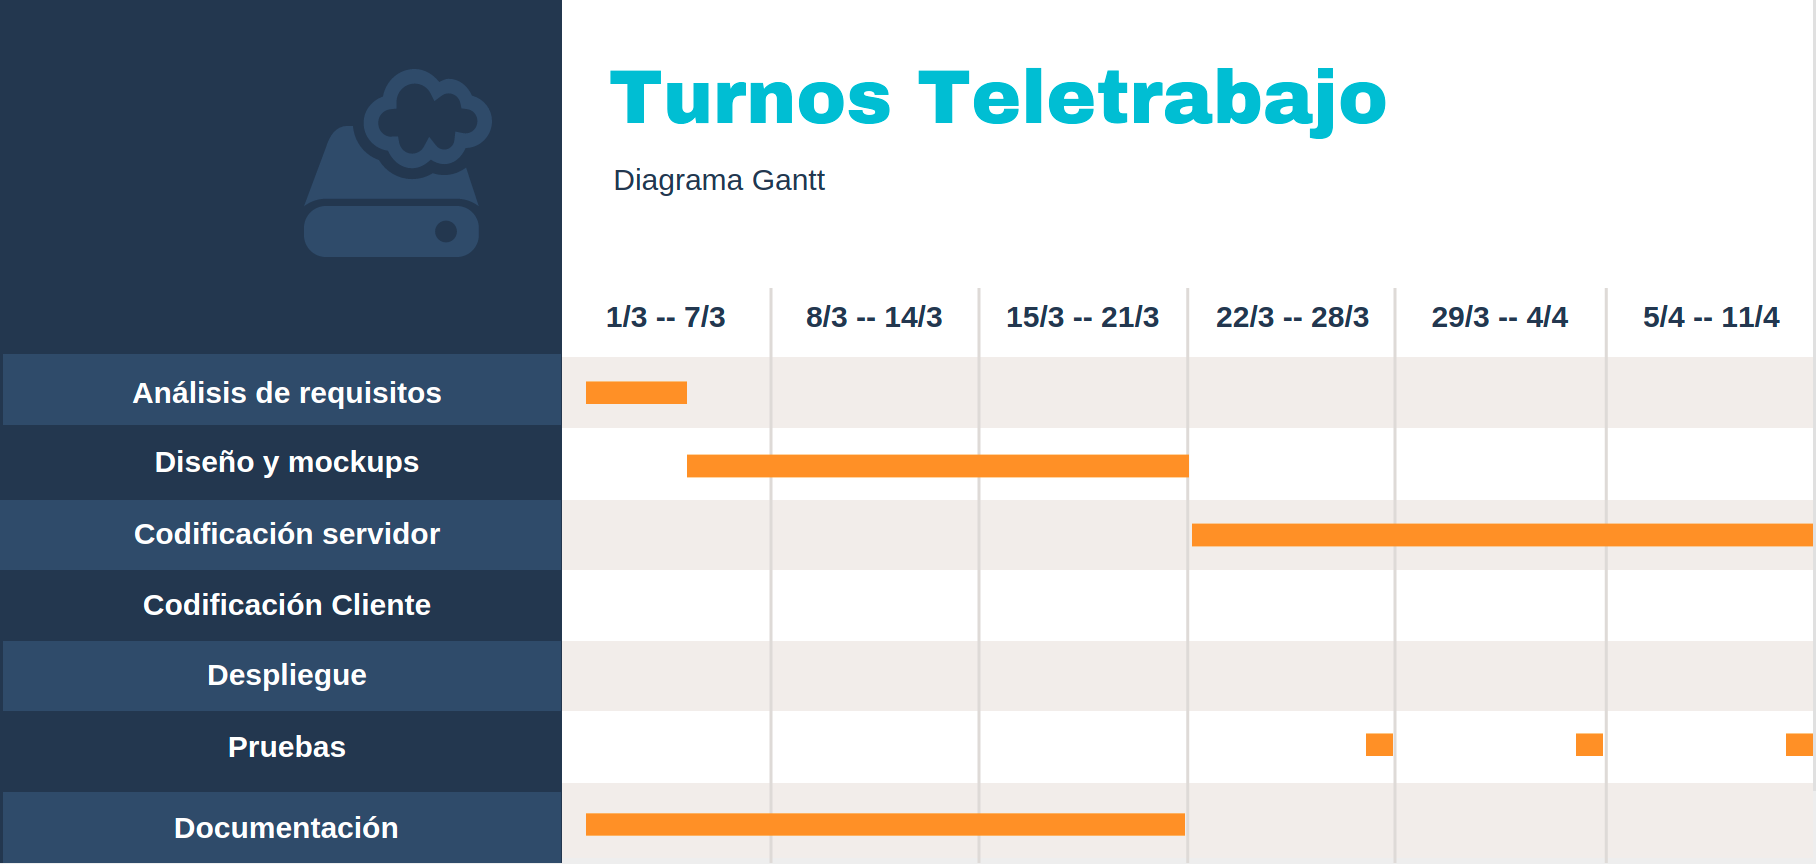
\includegraphics[width=\linewidth]{img/gantt1.png}[h!] % [h!]
   \caption{Primer segmento Gantt}
   \label{fig:Gantt1}
 \end{figure}

 \begin{figure}
   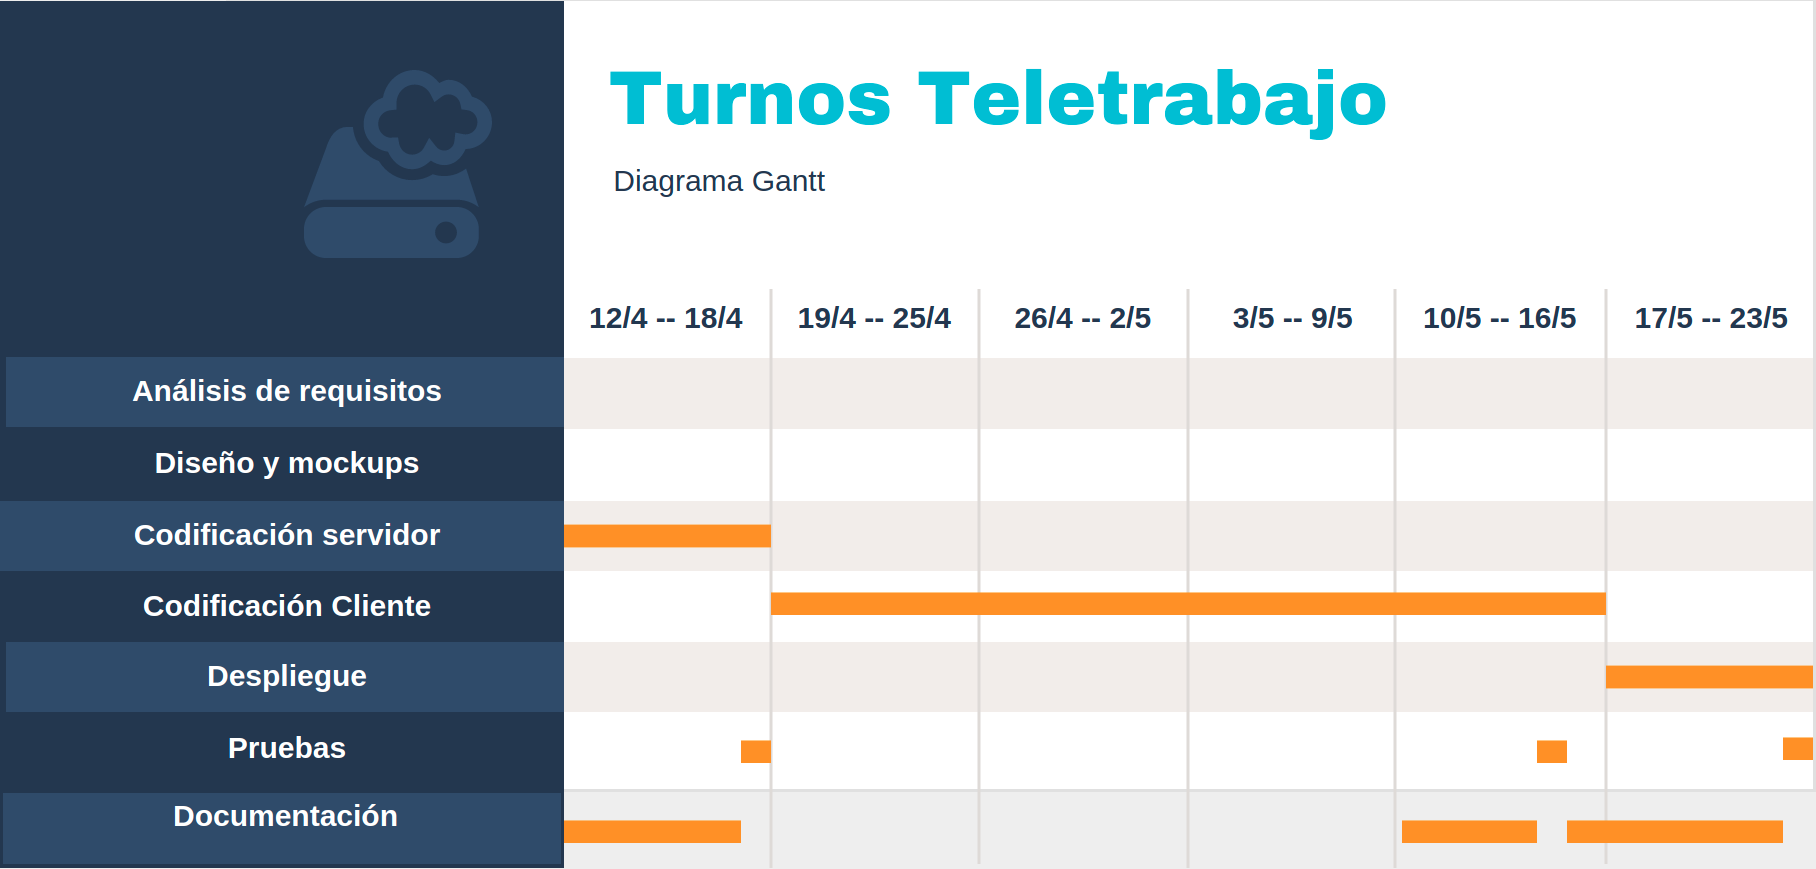
\includegraphics[width=\linewidth]{img/gantt2.png}[h!] % [h!]
   \caption{Segundo segmento Gantt}
   \label{fig:Gantt21}
 \end{figure}

\begin{itemize}
   \item Analisis de requisitos  (3 día)  
   \item Diseño y mockups ( 18 días)
   \begin{itemize}
      \item Diseño arquitectura
      \item Mockups
      \item Diagrama de componentes
      \item Diagrama mysql
      \item Mapa web
   \end{itemize}
   \item Codificación entorno servidor (28 días)
   \begin{itemize}
      \item Creación modelos sequelize
      \item Implementar autenticación
      \item Creación de rutas
      \item Pruebas Postman
   \end{itemize}
   \item Codificación entorno cliente (28 días)
   \begin{itemize}
      \item Autenticación
      \item Calendario
      \item Personalización
      \item Informes
      \item Panel administrador
   \end{itemize}
   \item Despliegue ( 7 días)
   \begin{itemize}
      \item Creación de contenedores
      \item Despliegue servidor dedicado
      \item Despliegue Google Gloud
      \item Pruebas de funcionamiento
   \end{itemize}
   \item Documentación ( 14 días a lo largo del proyecto)
   \item Optimización de código (7 días )
   \begin{itemize}
      \item Eliminación de posibles bugs
      \item Eliminación de mensajes en consola
      \item Optimización de código
   \end{itemize}
\end{itemize}

\chapter{Análisis de requisitos}

????? ????????????? ????????????? ????????????? ????????????? ????????????? 

\section{?? ???? ???? ? ?? ??}

????? ????????????? ????????????? ????????????? ????????????? ?????????????

\chapter{Diseño}

????? ????????????? ????????????? ????????????? ????????????? ????????????? 

\section{Diseño Conceptual Entidad Relación}

????? ????????????? ????????????? ????????????? ????????????? ?????????????

\section{Diseño Lógico Relacional o Paso a tablas}

????? ????????????? ????????????? ????????????? ????????????? ?????????????

\section{Diseño Físico o Diagrama Mysql}

????? ????????????? ????????????? ????????????? ????????????? ?????????????

\section{Orientación a objetos}

????? ????????????? ????????????? ????????????? ????????????? ?????????????

\section{Mapa Web}

????? ????????????? ????????????? ????????????? ????????????? ?????????????

\section{Mockups}

????? ????????????? ????????????? ????????????? ????????????? ?????????????

\chapter{Codificación}

\section{Tecnologías elegidas y su justificación}

Se ha usado yaml para el fichero de configuración de docker-compose y las acciones de github, \LaTeX{} se ha usado para crear la documentación, siendo ambos lenguajes de marcas.
Se ha usado tanto para el frontend como para el backend el lenguaje Javascript, unificando ambos en un único lenguaje, facilitando el mantenimiento y el desarrollo al sólo tener que usar un único lenguaje.
En backend se ha usado la combinación de Node como motor de ejecución de javascript y Express como framework web, siendo una combinación muy usada para crear REST API, muy bien documentada.
Para el acceso a la base de datos he optado por usar el ORM Sequelize, que conjuntamente con el uso de promesas dota de funcionamiento ininterrumpido el backend. 
También realiza la función de prevenir la inyección de sql, si bien es cierto que en Sequelize 3.x y 5.x se descubrieron unas vulnerabilidades que permitían inyectar código sql en mariadb, se parchearon de forma definitiva en la versión 5.15.1, en el proyecto se ha usado la versión 6.6.2
Para la gestión de accesos y contraseñas se ha usado el paquete node jsonwebtoken (JWT), que es componente de uso común para gestionar las sesiones entre cliente y servidor, y para encriptar la contraseña se ha usado el módulo bcrypt.

En el frontend se ha usado Quasar, para poder generar una aplicación móvil e instalarla a través de herramientas MDM como SOTI, una aplicación de escritorio para los sistemas cerrados en los que no hay instalado un navegador, y la aplicación web de acceso común para el resto del personal.
Se ha usado la librería QCalendar de Quasar, que dota de funciones de fecha/hora, así como un interfaz de calendario mensual/semanal/diario.
Para el acceso a la parte cliente, se ha usado axios, que es el módulo que recomienda Quasar para las peticiones Ajax.
En la personalización de los usuarios adopté el módulo qiconpicker para elegir el icono personal y vue-html2pdf para imprimir el calendario. Vue-html2pdf es un componente basado en html2pdf, que te permite elegir el componente vue a imprimir directamente, su funcionalidad prácticamente es la misma que html2pdf.

He usado imagenes docker compatibles tanto con windows como con linux. Para esto he tenido que realizar algún sacrificio (buscar que era), pero la aplicación completa puede correr tanto en windows como en linux.
Se puede usar tanto el docker-compose suministrado como levantar los distintos contenedores en equipos distintos, sólo necesario configurar el fichero de cliente.

\section{Entorno servidor}
Node.js es un motor de ejecución JavaScript muy ligero, que puede realizar funciones de servidor web. 
En niveles de carga altos, está por debajo de nginx o apache, pero para las necesidades que tenemos para el API, es suficiente y rápido.
Se suele usar un servidor Nginx como proxy inverso al servidor node, en primera instancia no se va a implementar ya que el objetivo es que esté tanto cliente como servidor en el mismo equipo, unidos sólo por el tunel docker.
Sequelize es uno de los ORM más usados en JavaScript, securizando el acceso a los datos. 
JWT es un estándar para propagar la identidad del usuario identificado, necesario para poder realizar los distintos accesos a la API sin necesidad de crear sesiones.
La información está codificada en objetos JSON. 

Crear imagen de un token JWT (login-crea token-devuelve token --- Envia peticion con token-comprueba token-devuelve los datos pedidos)

\section{Entorno cliente}

Se ha usado el framework Quasar, basado en vue, para crear una SPA. 

También nos ha permitido crear la aplicación móvil y la de escritorio. En ambos casos, se ha usado de las librerías auxiliares Capacitor y Electron respectivamente.
Este framework nos permite crear de forma muy rápida interfaces de usuario. 
Las clases en los componentes Quasar funcionan prácticamente igual que Bootstrap para css, por lo que no ha habido prácticamente curva de aprendizaje.

\chapter{Despliegue}

El despliegue se ha realizado en un servidor privado, expuesto a internet en la siguiente dirección:
\url{https://}.

\section{Instalación de los archivos}

????? ????????????? ????????????? ????????????? ????????????? ?????????????

\chapter{Herramientas de apoyo}

Visual Studio Code como IDE.
Sonarqube para analizar la calidad del código.
Git como control de versiones.
Github Actions como CI/CD.
Docker y Docker Compose como entorno de virtualización.


\section{?? ???? ???? ? ?? ??}

????? ????????????? ????????????? ????????????? ????????????? ?????????????


%%%%%%%%%%%%%%%%%%%%%%%%%%%%%%%%%%%%%%%%%%%%%%%%%%%%%%%%%%%%%%%%%%%%%%%%%%%%%%%
%                                 CONCLUSIONS                                 %
%%%%%%%%%%%%%%%%%%%%%%%%%%%%%%%%%%%%%%%%%%%%%%%%%%%%%%%%%%%%%%%%%%%%%%%%%%%%%%%

\chapter{Conclusions}

????? ????????????? ????????????? ????????????? ????????????? ????????????? 

%%%%%%%%%%%%%%%%%%%%%%%%%%%%%%%%%%%%%%%%%%%%%%%%%%%%%%%%%%%%%%%%%%%%%%%%%%%%%%%
%                                BIBLIOGRAFIA                                 %
%%%%%%%%%%%%%%%%%%%%%%%%%%%%%%%%%%%%%%%%%%%%%%%%%%%%%%%%%%%%%%%%%%%%%%%%%%%%%%%

\begin{thebibliography}{10}

\bibitem{WAR}
   Issue del github de sequelize donde está la definición y ejemplos de clases para definir los modelos.
   \newblock Consultat a 
   \url{https://github.com/sequelize/sequelize/issues/6524}.

\bibitem{WAR}
   Howto creación de api con Node, Sequelize, Express y mysql.
   \newblock Consultat a 
   \url{https://bezkoder.com/node-js-express-sequelize-mysql}.

\bibitem{WAR}
   Documentación oficial sequelize.
   \newblock Consultat a 
   \url{https://sequelize.org/master}.

\bibitem{WAR}
   Documentación oficial sequelize.
   \newblock Consultat a 
   \url{https://sequelize.org/master}.

\bibitem{WAR}
   Documentación oficial componente QCalendar.
   \newblock Consultat a 
   \url{https://quasarframework.github.io/quasar-ui-qcalendar/docs}.

\bibitem{WAR}
   Documentación oficial Express.
   \newblock Consultat a 
   \url{https://expressjs.com/es/guide/routing.html}.

%%%%%%%%%%%%%%%%%%%%%%%%%%%%%%%%%%%%%%%%%%%%%%%%%%%%%%%%%%%%%%%%%%%%%%%%%%%%%%%
% MODEL D'ARTICLE                                                             %
%%%%%%%%%%%%%%%%%%%%%%%%%%%%%%%%%%%%%%%%%%%%%%%%%%%%%%%%%%%%%%%%%%%%%%%%%%%%%%%
\bibitem{light}
   Jennifer~S. Light.
   \newblock When computers were women.
   \newblock \textit{Technology and Culture}, 40:3:455--483, juliol, 1999.

%%%%%%%%%%%%%%%%%%%%%%%%%%%%%%%%%%%%%%%%%%%%%%%%%%%%%%%%%%%%%%%%%%%%%%%%%%%%%%%
% MODEL DE LLIBRE                                                             %
%%%%%%%%%%%%%%%%%%%%%%%%%%%%%%%%%%%%%%%%%%%%%%%%%%%%%%%%%%%%%%%%%%%%%%%%%%%%%%%
\bibitem{ifrah}
   Georges Ifrah.
   \newblock \textit{Historia universal de las cifras}.
   \newblock Espasa Calpe, S.A., Madrid, sisena edició, 2008.

%%%%%%%%%%%%%%%%%%%%%%%%%%%%%%%%%%%%%%%%%%%%%%%%%%%%%%%%%%%%%%%%%%%%%%%%%%%%%%%
% MODEL D'URL                                                                 %
%%%%%%%%%%%%%%%%%%%%%%%%%%%%%%%%%%%%%%%%%%%%%%%%%%%%%%%%%%%%%%%%%%%%%%%%%%%%%%%
\bibitem{WAR}
   Comunicat de premsa del Departament de la Guerra, 
   emés el 16 de febrer de 1946. 
   \newblock Consultat a 
   \url{http://americanhistory.si.edu/comphist/pr1.pdf}.

\end{thebibliography}
\cleardoublepage

%%%%%%%%%%%%%%%%%%%%%%%%%%%%%%%%%%%%%%%%%%%%%%%%%%%%%%%%%%%%%%%%%%%%%%%%%%%%%%%
%                           APÈNDIXS  (Si n'hi ha!)                           %
%%%%%%%%%%%%%%%%%%%%%%%%%%%%%%%%%%%%%%%%%%%%%%%%%%%%%%%%%%%%%%%%%%%%%%%%%%%%%%%

\APPENDIX

%%%%%%%%%%%%%%%%%%%%%%%%%%%%%%%%%%%%%%%%%%%%%%%%%%%%%%%%%%%%%%%%%%%%%%%%%%%%%%%
%                         LA CONFIGURACIO DEL SISTEMA                         %
%%%%%%%%%%%%%%%%%%%%%%%%%%%%%%%%%%%%%%%%%%%%%%%%%%%%%%%%%%%%%%%%%%%%%%%%%%%%%%%

\chapter{Configuració del sistema}

????? ????????????? ????????????? ????????????? ????????????? ?????????????

\section{Fase d'inicialització}

????? ????????????? ????????????? ????????????? ????????????? ?????????????

\section{Identificació de dispositius}

????? ????????????? ????????????? ????????????? ????????????? ?????????????

%%%%%%%%%%%%%%%%%%%%%%%%%%%%%%%%%%%%%%%%%%%%%%%%%%%%%%%%%%%%%%%%%%%%%%%%%%%%%%%
%                               ALTRES  APÈNDIXS                              %
%%%%%%%%%%%%%%%%%%%%%%%%%%%%%%%%%%%%%%%%%%%%%%%%%%%%%%%%%%%%%%%%%%%%%%%%%%%%%%%


\chapter{??? ???????????? ????}

????? ????????????? ????????????? ????????????? ????????????? ????????????? 



%%%%%%%%%%%%%%%%%%%%%%%%%%%%%%%%%%%%%%%%%%%%%%%%%%%%%%%%%%%%%%%%%%%%%%%%%%%%%%%
%                              FI DEL DOCUMENT                                %
%%%%%%%%%%%%%%%%%%%%%%%%%%%%%%%%%%%%%%%%%%%%%%%%%%%%%%%%%%%%%%%%%%%%%%%%%%%%%%%

\end{document}
